To the best of our knowledge, no proper weak error
analysis has been done in the rough volatility context. However, we try in Section  \ref{sec:Weak error analysis} to shortly discuss it in the context of the rBergomi and then in Section \ref{sec: choice of simulation scheme}, we explain how we choose the optimal simulation scheme for the optimal performance of our approach.
\subsection{Weak error analysis}\label{sec:Weak error analysis}
In this work, we are interested in approximating $\expt{g(X_T}$, where $g$ is some smooth function and $X$ is the asset price under the rBergomi dynamics such that $X_t=X_t(W^{(1)}_t,\widetilde{W}_t)$ where $W^{(1)}$ is standard Brownian motion and  $\widetilde{W}_t$ is the fractional Brownian motion as given by \eqref{eq:Volterra process}.  Then we can express the approximation of $\expt{g(X_T}$  using the  hybrid and exact schemes as the following 
\begin{align*}
\expt{g\left(X_T\left(W^{(1)}_t,\widetilde{W}_t \right)\right)} \approx \expt{g\left(\overline{X}_N\left(W^{(1)}_1,\dots,W^{(1)}_N, \overline{W}_1, \dots,\overline{W}_N\right)\right)}:\quad \textbf{(Hybrid  scheme)},
\end{align*}
\begin{align*}
\expt{g\left(X_T\left(W^{(1)}_t,\widetilde{W}_t\right)\right)} \approx \expt{g\left(\overline{X}_N\left(W^{(1)}_1,\dots,W^{(1)}_N, \widetilde{W}_1, \dots,\widetilde{W}_N\right)\right)}:\quad \textbf{(Exact  scheme)},
\end{align*}
where $\overline{W}$ is the approximation of $\widetilde{W}$  as given by \eqref{eq:Hybrid_scheme_pre} and $\overline{X}_N$ is the approximation of $X$ using $N$ time steps.

To simplify notation, let  $\overline{\mathbf{W}}=(\overline{W}_1,\dots,\overline{W}_N)$, $\mathbf{W}^{1}=(W^{(1)}_1,\dots,W^{(1)}_N)$ and $\widetilde{\mathbf{W}}=(\widetilde{W}_1,\dots,\widetilde{W}_N)$. If we denote by $\mathcal{E}_{B}^{Hyb}$ and $\mathcal{E}_{B}^{Chol}$ the weak errors produced by the hybrid and Cholesky scheme respectively, then we can write
\begin{small}
\begin{align}\label{eq: Weak_error_hyb_chol}
\mathcal{E}_{B}^{Hyb}&=\abs{\expt{g\left(X_T\left(W^{(1)}_t,\widetilde{W}_t\right) \right)}-\expt{g\left(\overline{X}_N\left(\mathbf{W}^{1}, \overline{\mathbf{W}}\right) \right)}} \nonumber\\
&\le \abs{\expt{g\left(X_T\left(W^{(1)}_t,\widetilde{W}_t\right)\right)}-\expt{g\left(\overline{X}_N\left(\mathbf{W}^{1}, \widetilde{\mathbf{W}}\right)\right)}}+ \abs{ \expt{g\left(\overline{X}_N\left(\mathbf{W}^{1}, \overline{\mathbf{W}}\right)\right)}- \expt{g\left(\overline{X}_N\left(\mathbf{W}^{1}, \widetilde{\mathbf{W}}\right)\right)}}\nonumber\\
&\le \mathcal{E}_{B}^{Chol}+ \abs{ \expt{g\left(\overline{X}_N\left(\mathbf{W}^{1}, \overline{\mathbf{W}}\right)\right)}- \expt{g\left(\overline{X}_N\left(\mathbf{W}^{1}, \widetilde{\mathbf{W}}\right)\right)}}
\end{align}
\end{small}
From the construction of the Cholesky scheme, we expect that the weak error is purely the discretization error, that is
\begin{align*}
\mathcal{E}_{B}^{Chol}=\Ordo{\Delta t},
\end{align*}
which was confirmed by our numerical experiments (for illustration see Figure \ref{fig:set1_weak_rate_exact} for the case of Set $1$  in Table \ref{table:Reference solution, using MC with $500$ time steps, of Call option price under rBergomi model, for different parameter constellation.}). 

The second term in \eqref{eq: Weak_error_hyb_chol} is basically related to approximating the integral \eqref{eq:Volterra process}  by \eqref{eq:Hybrid_scheme}. From our numerical experiments it seems that that term is also of order at least $\Delta t$  and its rate of convergence is independent of $H$ (for illustration see Figure \ref{fig:set1_weak_rate_hybrid} for the case of Set $1$  in Table \ref{table:Reference solution, using MC with $500$ time steps, of Call option price under rBergomi model, for different parameter constellation.}).

\FloatBarrier
\begin{figure}[h!]
	\centering
	\begin{subfigure}{.5\textwidth}
		\centering
		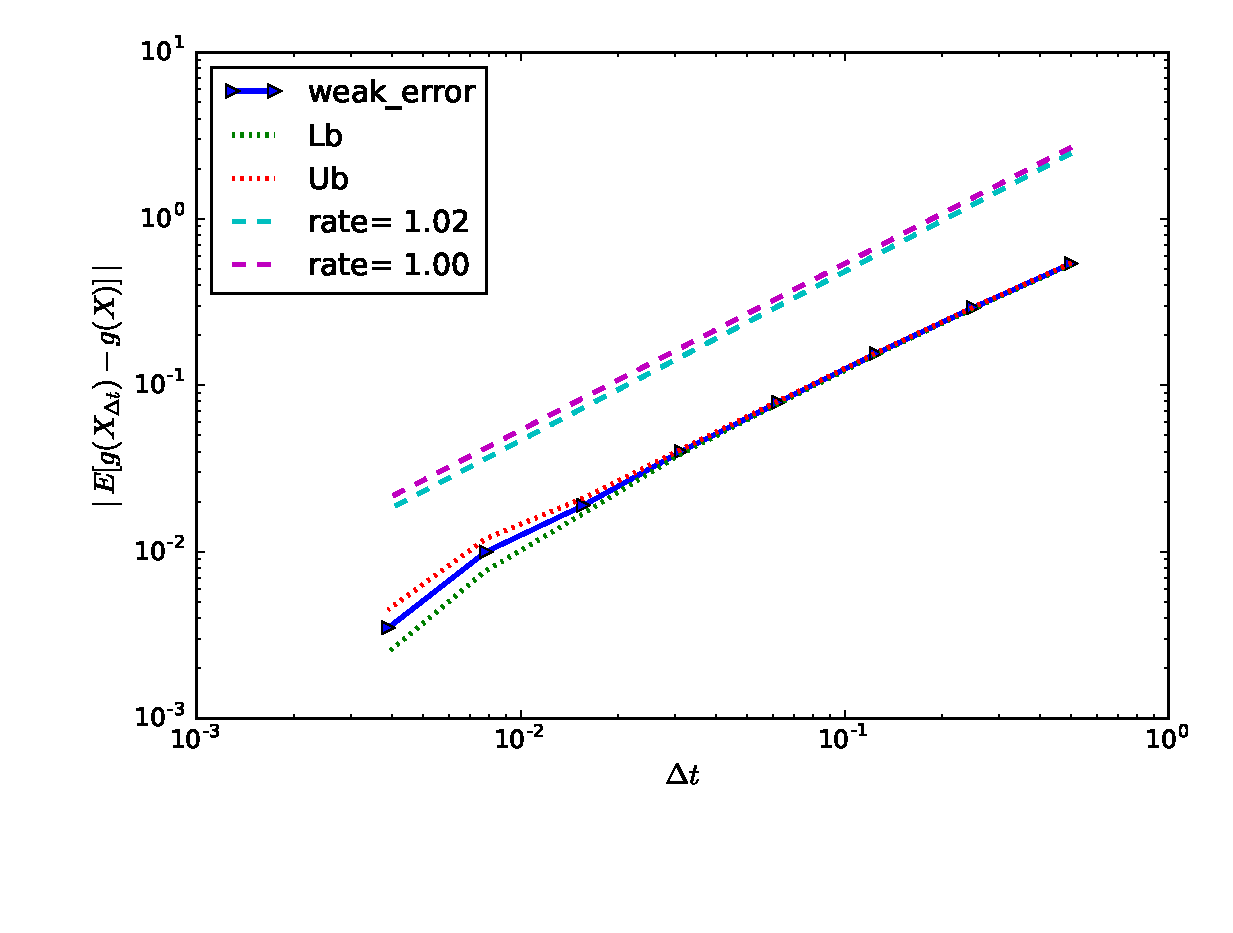
\includegraphics[width=1\linewidth]{./figures/rBergomi_weak_error_rates/without_richardson/H_007/weak_convergence_order_Bergomi_H_007_K_1_M_4_10_6_CI_relative_hybrid_non_hierarchical_non_parallel_asymptotic}
		\caption{}
		\label{fig:set1_weak_rate_hybrid}
	\end{subfigure}%
	\begin{subfigure}{.5\textwidth}
		\centering
		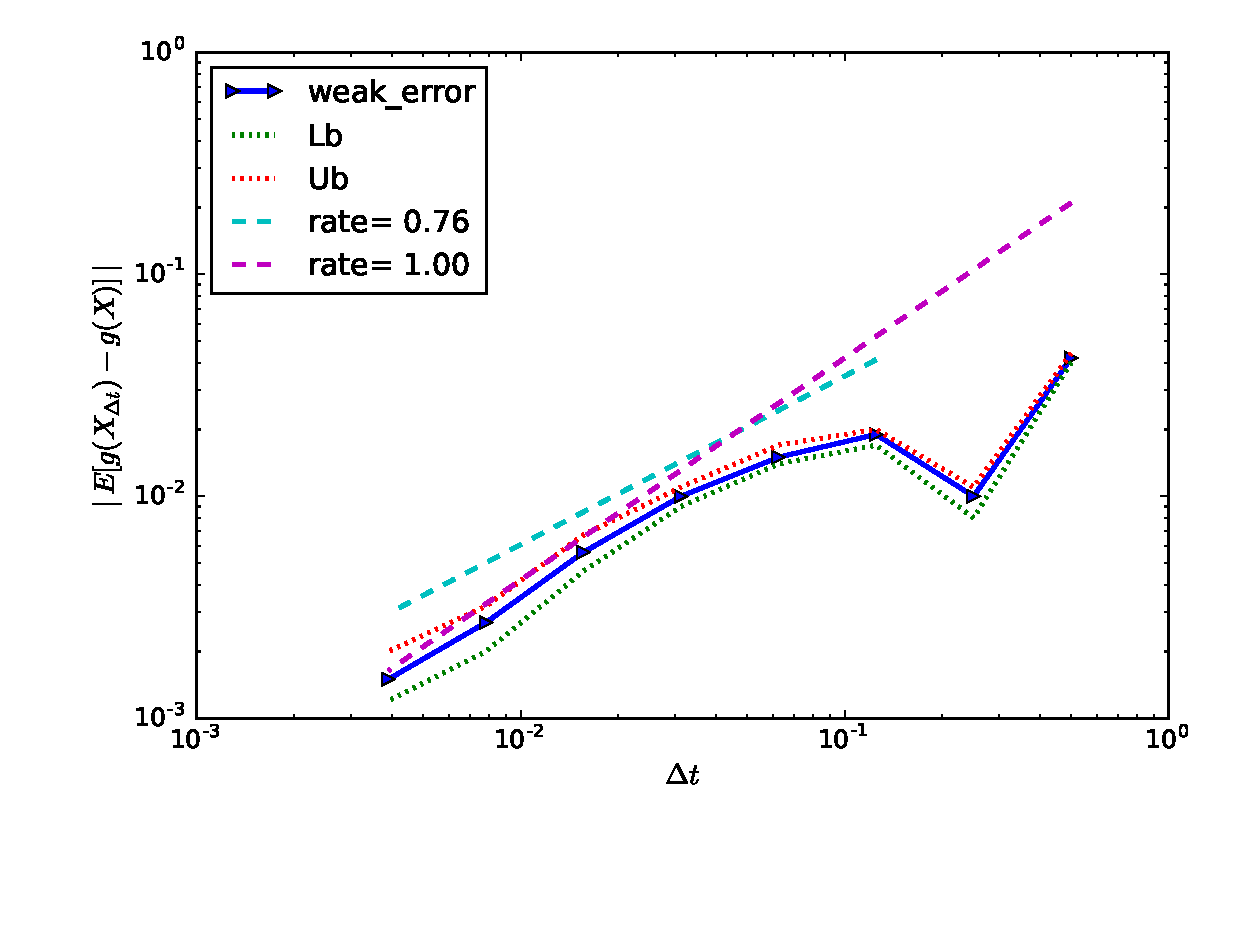
\includegraphics[width=1\linewidth]{./figures/rBergomi_weak_error_cholesky/weak_convergence_order_Bergomi_H_007_K_1_M_4_10_6_CI_relative_cholesky_non_hierarchical_non_parallel_asymptotic}
		\caption{}
		\label{fig:set1_weak_rate_exact}
	\end{subfigure}
	\caption{The convergence of the weak error $\mathcal{E}_B$, using MC with $6 \times 10^6$ samples, for Set $1$ parameter in Table \ref{table:Reference solution, using MC with $500$ time steps, of Call option price under rBergomi model, for different parameter constellation.}. We refer to $C_{\text{RB}}$ (as in \eqref{BS_formula_rbergomi}) for $\expt{g(X)}$, and to $C_{\text{RB}}^{N}$ (as in \eqref{BS_formula_rbergomi_2}) for $\expt{g(X_{\Delta t})}$. The upper and lower bounds are $95\%$ confidence intervals. a) With the hybrid scheme  b) With the exact scheme.}
	\label{fig:Weak_rate_set1_set_2_without_rich_hyb+chol}
\end{figure}
\FloatBarrier
\subsection{On the choice of the simulation scheme in our approach}\label{sec: choice of simulation scheme}
The choice of the simulation scheme in our approach was based on the observed behavior of the weak rates. Through our numerical experiments (see Table \ref{table:Reference solution, using MC with $500$ time steps, of Call option price under rBergomi model, for different parameter constellation.} for the tested examples), we observe that although the hybrid and exact schemes  converge asymptotically with weak rate of $\Ordo{\Delta t}$, the pre-asymptotic behavior of the weak rate is different for both schemes. As an illustration, from Figure \ref{fig:Weak_rate_set1_set_2_without_rich_hyb+chol} for Set $1$ parameter in Table \ref{table:Reference solution, using MC with $500$ time steps, of Call option price under rBergomi model, for different parameter constellation.}, the hybrid scheme  has a consistent convergence behavior in the sense that it behaves in the asymptotic way basically right from the beginning, whereas the exact scheme does not. On the other
hand, the constant  seems considerably smaller for the exact scheme. These two features  makes the hybrid scheme the optimal scheme  to work with in our context since our approach is based on hierarchical transformations involving the use of Richardson extrapolation (see Section \ref{sec:Richardson extrapolation}).